%----------- Capítulo 3: Especificação do Software -------------

\chapter{Especificação do Software}
O software em questão consiste em um serviço web que tem como principal funcionalidade responder a rota entre dois pontos informados com menor tempo de viagem utilizando o sistema de transporte público. 
Nas seções a seguir serão apresentados os requisitos do sistema bem como sua arquitetura.

\section{Requisitos do Sistema}
A seguir estão listadas os requisitos do sistema.

\subsection{Requisitos Funcionais}
\begin{itemize}
	\item O software deverá retornar para o usuário a rota com menor tempo de viagem entre dois pontos informados.
	\item O software deverá mostrar a rota resultante desenhada em um mapa, diferenciando as linhas de transporte por cor, e também no formato texto como uma sequência de passos.
	\item O software deverá receber do usuário os pontos de partida/destino no formato de endereço e/ou marcando-os no mapa.
	\item O software deverá receber o horário de partida no formato HH:MM.
	\item O software deverá funcionar independente de qual fonte de dados for escolhida, contudo que esta respeite o padrão GTFS.
\end{itemize}

\subsection{Requisitos Não-Funcionais}
\begin{itemize}
	\item O software deverá ser disponibilizado como livre, possibilitando futuras contribuições.
	\item O software deverá ser disponibilizado no formato de um serviço web.
	\item O software devera utilizar o padrão GTFS para o arquivo fonte de dados contendo as rotas do sistema público de transporte de determinada cidade.
	\item O software deverá ser desenvolvido em linguagem Java e, para o núcleo web, javascript.
	\item O software deverá utilizar um banco de dados de grafos para armazenamento das rotas do sistema de transporte público.
\end{itemize}

\section{Arquitetura do Sistema}
O sistema em questão é composto de quatro núcleos principais: Core, GTFS Importer, Web Service e Cliente. 
O fluxo padrão do sistema como um todo é mostrado na \ref{fig:arquitetura}.
Primeiramente o usuário informa os pontos de origem e destino para o Cliente através do mapa ou fornecimento do endereço por extenso. 
Feito isso, os dados coletados são enviados ao Web Service através de um HTTP POST. 
Este responsável pela execução da query para encontrar a rota contendo o caminho mínimo através do acesso ao banco de dados com os métodos e entidades contidas no Core.
Ao terminar de executar a query no banco, o Web Service responde ao Cliente as informações sobre a rota resultantes através de um objeto serializado no formato JSON, sendo este responsável por mostrá-las para o usuário visualmente através de um mapa.
Para que qualquer consulta seja bem sucedida, é necessário que o banco de dados esteja populado com as informações do arquivos no padrão GTFS, o que é realizado através do núcleo GTFS Importer.
A seguir uma explicação detalhada de cada módulo do sistema.

\begin{figure}[!htb]
	\centering
	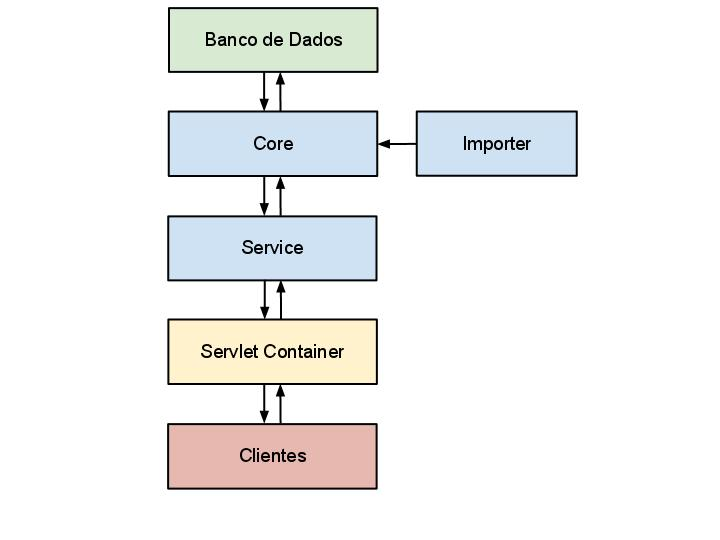
\includegraphics[width=1\textwidth]{./arquitetura.jpg} % <- formatos PNG, JPG e PDF
	\caption[ImgArquitetura]{Visão geral da arquitetura do sistema.}
	\fonte{Autoria Própria}
	\label{fig:arquitetura}
\end{figure}

\subsection{Core}
Este módulo contém todas as representações das entidades presentes nos arquivos GTFS

\subsection{GTFS Importer}

\subsection{Web Service}

\subsection{Cliente Web}

\section{Considerações}

